Dette kapitel vil beskrive todimensionale vektorer som 2-vektorer, og tredimensionelle vektorer som 3-vektorer.
Der vil blive brugt bracket notation for vektorer.
Det er her fordelagtigt at introducere Det Euklidiske Rum.
\begin{frdef}[Det Euklidiske Rum]\label{def:euklid_rum}
	Det Euklidiske Rum, nogle gange kaldet det Kartesianske rum, eller $\mathbf{n}$-rummet, er rummet, der indeholder alle n-tupler, af reelle tal ($\set{x_1,x_2,\dots,x_n}$).
$\mathbb{R}^n$ er derfor et vektorrum, og betegnes også som n-vektorer.
Derved har man at $\mathbb{R}^1=\mathbb{R}$, $\mathbb{R}^2$ er Den Euklidiske Plan.
\end{frdef}

Det fremkommer af Det Euklidiske Rum, at en 4-vektor, kan skrives som $\mathbb{R}^4$.
Dette er da Definition \ref{def:euklid_rum} siger, at n-vektorer, skal være $\mathbb{R}^n$.

\begin{frdef}[Vektorer]
	En vektor er i geometrien et objekt, der er defineret ved at have en længde og en retning.
\end{frdef}

\section{Geometrien i sæt af vektorer}
Dette afsnit har til formål at beskrive det geometriske aspekt af vektorer.
Det vil dække spænding af vektorer.

\subsection{Spændinger af vektorer over $\mathbb{R}$}
 
\begin{equation}
	\mathrm{Span}\{v\}=\set*{\alpha v; \alpha\in\mathbb{R}}
\end{equation}

Ovenstående er et sæt, der kun indeholder lineære kombinationer, af en ikke-nul-vektor $v$.
Hvis et tomt sæt af 2-vektorer skal beskrives, findes en vektor i sættet, en nul-vektor.
Denne vektor er beskrevet som $[0,0]$, i vektor notation.

Samtidig beskriver det ovenstående sæt også, at der for en 2-vektor, findes uendelig mange punkter i eksempelvis $\set*{\alpha[2,3]; \alpha\in\mathbb{R}}$, hvor vektoren kan 

I en spænding af $\set{[1,0],[0,1]}$, er de to vektorer standard for $\mathbb{R}^2$, hvorved hver 2-vektor er i spændingen.
Dette betyder at sættet indeholder alle punkter i Den Euklidiske Plan.

En 4-vektor kan også betegnes som et sæt af elementer eller en funktion.
Betragt følgende vektor $\set{2.87,6.2,3.7,1.5}$.
Dette kan betegnes som funktionen
\begin{align}
	\label{eqn:vec_func}
	0&\mapsto 2.87\\
	1&\mapsto 6.2\\
	2&\mapsto 3.7\\
	3&\mapsto 1.5
\end{align}

Samme 4-vektor kan repræsenteres som en Python Dictionary $\set{0:2.87, 1:6.2, 2:3.7, 3:1.5}$.

\subsection{Sparsitet}
En vektor hvis værdier alle er 0, kaldes en sparsom eller nul-vektor.
Hvis ikke mindre end $k$ værdier i vektoren er 0, kaldes vektoren en k-sparsom vektor.
Vektorer der repræsenterer data, der er opsamet af sensorer, er næste aldrig sparsomme vektorer.

\section{Hvad kan vises med vektorer}
Mange ting kan vises med vektorer.
Blandt disse ting er \emph{Binære strenge}, altså strænge at 1 og 0, der har en given værdi.
Disse vises ved vektorer som $\set{1,0,0,1,1,0,1}$, hvor vektoresn længde, er det samme som længden af den binære streng.
\emph{Attributer} kan også vises med vektorer.
Dette er som vist i \cref{eqn:vec_func}, hvor to værdier kan sidestilles som en Python Dictionary.
Mere relevant for sandsynlighedsteori, kan vi også repræsenterer \emph{Sandsynligheds distribution} med vekoterer.
Dette vises igen som i \cref{eqn:vec_func}, hvor hver key er mapped til en værdi.
\emph{Billeder} kan også vises som vektorer, da hvor farve har en RGB værdi, som kan afkodes til en binær værdi.
Ydermere kan punkter i rummet plottes som vektorer, dog er dette givet ved Mat A adgangskursus, så dette behøver ikke yderligere forklaring.


\section{Vektor addition}\label{sec:addition}
Vektor addition foregår som på Mat A adgangskurset.
Dog vil denne sektion gå mere i dybten med vektor addition.


\begin{frdef}[KLEIN s.
69]
	Addition af n-vekoterer er definieret ved addition af de respektive værdier.\\
	$[u1,u2,u3] + [v1,v2,v3] = [u1+v1, u2+v2, u3+v3]$
\end{frdef}

Siden vektorer som $[1,2]$ kan bruges som et opslag, kan den tænkes som at overføre en værdi.
Eksempelvis fra $[4,4]$ til $[5,6]$.
Derfor må den også kunne adderes.

Samtidig findes der regler for addition af vektorer, eksempelvis at
\begin{equation}
	x+y=y+x
\end{equation}
Samt
\begin{equation}
	(x+y)+z=x+(y+z)
\end{equation}
\section{Skalarproduktet}\label{sec:scalar}
Ligesom med addition er dette også gennemgået på Mat A adgangskurset.
Multiplikation af en vektor, med en skalar $\alpha$, svarer til at gange på hver værdi i vektoren.
Dette kan eksemplificeres med vektoren $[3,4,7]$.
Hvis denne ganges med skalaren 5, gøres dette på følgende vis:
\begin{equation}
	\label{eqn:scalar}
	5[3,4,7] = [5\cdot3,5\cdot4,5\cdot7] = [15,20,35]
\end{equation}
Hvis der samtidig adderes en vektor på, følger dette de arritmetiske regler. 
Der ganges først, så adderes der.
Hvis en vektor ganges med et negativt tal, ændres fortegnet for alle elementer i vektoren.
Dette betyder at vektoren vil ændre orientering.
Samtidig gælder følgende for multiplikation af vektorer med ekstra skalarer:
\begin{equation}
	\label{eqn:scalar_mult}
	\alpha(\beta v)=(\alpha\beta)v
\end{equation}

\subsection{Linjer gennem origo}\label{ssec:lto}
Med vektorer kan linjer også tegnes fra origo.
Dette kan blandt andet gøres med følgende sæt af punkter.
\begin{equation}
	\label{eqn:origo}
	\set*{\alpha v; \alpha\in\mathrm{R},0\leq\alpha\leq1}
\end{equation}
Ovenstående sæt tenger en linje af punkter fra origo til $v$.
Med python koden vist i \cref{lst:python_plot} gives følgende plot
\begin{figure}[h]
	\centering
	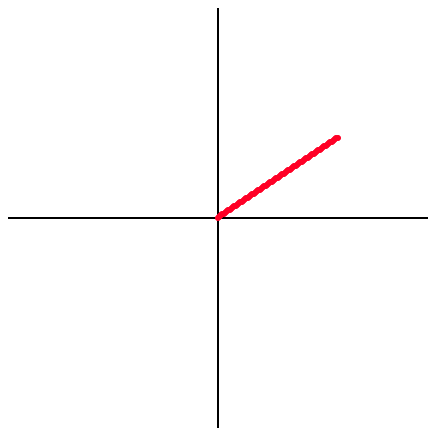
\includegraphics[width=0.5\textwidth]{img/vecplot.png}
	\caption{Plot fra udsnittet \cref{lst:python_plot}}
	\label{fig:plot_line}
\end{figure}
\lstinputlisting[
	language=Python,
	firstline=4,
	lastline=7,
	firstnumber=4,
	label=lst:python_plot,
	caption={Python kode til at generere plot i \cref{fig:plot_line}.\\Koden kan findes i ./labs/vectors/python\_plot.py}
]{labs/vectors/python_plot.py}

I kombination med at segmenter af linjer, kan samles til hele linjer og at der kan dannes uendelig mange skalar vektorer, kan vi danne figurer, når $\alpha$ strækker sig over flere tal.
Skalarprodukter $<1$ giver anledning til kopier af $v$, samtidig med at negative Skalarprodukter giver anledning til vektorer der peger i den anden retning.
Sættet af punkter $\set*{\alpha v;\alpha\in \mathrm{R}}$ strækker sig fra $-\infty;\infty$, og producerer derfor følgende plot:
\begin{figure}[h]
	\centering
	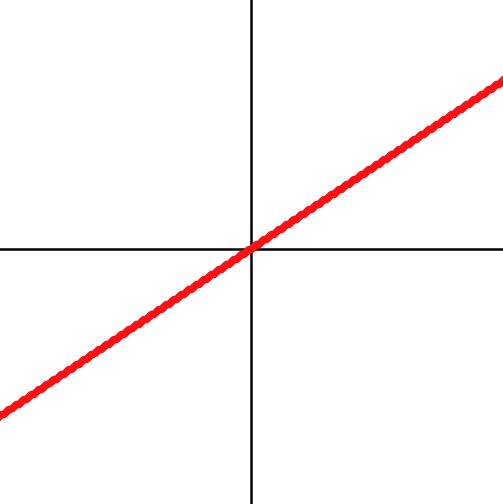
\includegraphics[width=0.5\textwidth]{img/thrh_origin.png}
	\caption{Sættet $\set*{\alpha v;\alpha\in \mathrm{R}}$ plottet i en graf.
	Både $x$ og $y$ aksen går fra $-\infty;\infty$}
	\label{fig:plot_through}
\end{figure}

Grafen i \cref{fig:plot_through} kan laves med følgende stykke python kode:
\lstinputlisting[
	language=Python,
	firstline=4,
	lastline=7,
	firstnumber=4,
	label=lst:scalar_plot,
	caption={Python kode til at generere plot i \cref{fig:plot_through}.\\Koden kan findes i ./labs/vectors/scalar\_plot.py}
]{labs/vectors/scalar_plot.py}

\section{Kombination af addition og skalar}
Med information fra \cref{sec:addition,sec:scalar,ssec:lto} kan det dedukteres at man med vektorer kan plotte alverdens figurer.
Dette betyder selvfølgelig også at man kan begynde at lege med mere avancerede former for vektore beregning.
Betragt nedenstående 

<<<<<<< HEAD
\section{Egenvektor}
En egenvektor er findes, hvis vektor-matrice produktet ikke er 0, efter multiplikation.
For fælgende eksempel findes det at der er tale om en egenvektor, da produktet ikke er 0:
\begin{equation}
    \left[
        \begin{matrix}
            1\\
            0\\
            -1
        \end{matrix}
    \right]
    \cdot
    \left[
        \begin{matrix}
            -1&-1&3\\
            -1&3&-1\\
            3&-1&-1
        \end{matrix}
    \right]
    =
    \left[
        \begin{matrix}
            -4\\
            0\\
            4
        \end{matrix}
    \right]
\end{equation}
Da produktet ikke er en nulvektor, kan det konkluderes at vektoren, der ganges på, er en egenvektor.

=======
\section{Vektorrum}
Først defineres $\mathcal{V}$ som et Vektorrum.
$\mathcal{V}$ har følgende egenskaber:
\begin{enumerate}
    \item $\mathcal{V}$ indeholder en nul-vektor
    \item For hver vektor $v$, hvis $\mathcal{V}$ indeholder $v$, indeholder den også $\alpha v$ for hver scalar $\alpha$
    \item For hvert par $u$ og $v$ af vektorer, hvis $\mathcal{V}$ indeholder $u$ og $v$, indeholder dette også $u+v$
\end{enumerate}
For ovenstående tre egenskaber kaldes disse V$n$.
\begin{frdef}
    Et sæt $\mathcal{V}$ af vektorer kaldes et vektorrum, hvis det overholder ovenstående tre egenskaber.
\end{frdef}
Udtrykket i V2 udtrykkes matematisk som ``$\mathcal{V}$ is \textit{closed under} scalar-vector multiplication.''
Ligeledes udtrykkes V3 som ``$\mathcal{V}$ is \textit{closed under} addition.''
\begin{frdef}
    Et vektorrum der kun består af en nul-vektor, kaldes et \textit{trivielt} vektorrum.
\end{frdef}

\subsection{Subrum}
\begin{frdef}
    Hvis $\mathcal{V}$ og $\mathcal{W}$ er vektorrum, og $\mathcal{V}$ er et subset af $\mathcal{W}$, siges det om $\mathcal{V}$ at være et Subrum af $\mathcal{W}$.
\end{frdef}
Det kan derfor vises at sættet $\set{[0,0]}$ (Det trivielle vektorrum), er et subset af $\set{\alpha[2,1];\alpha\in\mathbb{R}}$ og dermed også et subset af $\mathbb{R}^2$.
Ydermere er $\mathbb{R}^2$ det største subset af $\mathbb{R}^2$.

\subsection{Affine vektorrum}
Det afine vektorrum indeholder vektorer, der ikke går igennem oregon.
Dette skrives matematisk som $\set{a+v;v\in\mathcal{V}}$.
Dette kan omskrives til $a++\mathcal{V}$.


\section{Lineære systemer, homogene og andet}

\section{Practice Problems}
Dette afsnit vil behandle de givne opgaver fra forelæsnignerne til kapitlet.
\subsection{Problem 2.14.1}
Kursusgang 4.\\
For vectors $v=[-1,3]$ and $u=[0,4]$, find the vectors $v+u, v-u$ and $3v-2u$.
\begin{figure}[h]
    \centering
    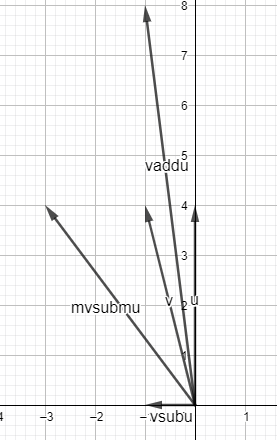
\includegraphics[]{img/vecfield2141}
    \label{ex:2141}
    \caption{Det genererede vektorfelt}
\end{figure}
De givne vektorer kan udregnes som vist i \cref{sec:addition}.
Vektorerne skal læses som $v$ add $u$ og $v$ sub $u$, hvor $m$ betyder multiplikation.
\subsection{Problem 2.14.2}
Kursusgang 4.\\
Given the vectors $v=[2,-1,5]$ and $u=[-1,1,1]$ find the vectors $v+u$, $v-u$, $2v-u$, and $v+2u$
\begin{equation}
    v+u=[1,0,6]
\end{equation}
\begin{equation}
    v-u=[3,-2,4]
\end{equation}
\begin{equation}
    2v-u=[5,-3, 9]
\end{equation}
\begin{equation}
    v+u+u=[0,1,7]
\end{equation}

\subsection{Problem 2.14.3}
Kurssusgang 4.\\
Here are six 7-vecotrs over $GF(2)$:
\begin{table}[h]
    \centering
    \begin{tabular}{|l|l|}
        \hline
        a=1100000&d=0001100\\
        b=0110000&e=0000110\\
        c=0011000&f=0000011\\\hline
    \end{tabular}
    \label{tab:fields}
    \caption{six 7-vectors}
\end{table}
For each of the following vectors $u$, find a subset of the above vectors whose sum is $u$, or report nu such subset exists.
\begin{enumerate}
    \item $u=0010010$
    \item $u=0010010$
\end{enumerate}
Vektor 1. kan dannes ved følgende kombination
\begin{equation}
    u==c+e+d=0011110
\end{equation}
Vektor 2. kan dannes ved følgende kombination
\begin{equation}
    u==b+c+d+e=0100010
\end{equation}
\subsection{Opgave til kapitel 2}
Kursusgang 4.\\
Lad  $D={'x', 'y', 'z'}$. 
Betragt vektorer i  $\mathbb{R}^D$ givet ved følgende dictionaries: $u=\set{x:3,z:-2}$, $v=\set{y:5,z:4}$, $w={x:2,z:3,y:4}$.
Udregn $u+v$ og $2w-u$
\begin{equation}
    u+v=\set{x:3,y:5,z:2}
\end{equation}
\begin{equation}
    2w-u=\set{x:1,y:8,z:8}
\end{equation}

>>>>>>> 38997c460ab79ca22c1ca90fb2fbbd43c4a90004
